\chapter{Implementation}

\paragraph{}
This section presents the work that has been done on the implementation.
We start by touching a few words on which variations have been used and what has been done before implementing our algorithm in parallel.
After that, we explicit each step of the parallel implementation, what has been implemented by hand and the parts that come from a library.
Finally, we present our experiments, the results and discuss them.

\section{Algorithm details}
\paragraph{Variations}
In our algorithm, we use spatially uniform sampling for the ease of implementation and robustness.
The kernel function is the bilateral function with the spatial parameter \(h_x = 40\) and the color intensity parameter \(h_z = 30\) (see section \ref{variations:affinity_functions}).
We use the re-normalised Laplacian \(\Lapl = \alpha (D-K)\) from \cite{milanfar_new_2016} to avoid expensive computation and use a simple definition.

\paragraph{Prototyping}
In the initial phase of the project, we implemented the algorithm proposed by \cite{glide_2014} in Python, using Numpy, in order to understand the mechanisms and issues of global filtering.
Needless to say that this implementation is sequential and limited to small images that require only little computational resources.


\section{Parallel implementation}
\paragraph{}
To scale our algorithm to use usual camera pictures, but also much larger inputs, we implemented it in a parallel manner using the C language and the Portable, Extensible Toolkit for Scientific Computation (PETSc) \cite{petsc_web_page}.
This library is built upon the message passing interface (MPI) and contains distributed data structures and parallel scientific computation routines.
\ifthesis
 The most useful are the matrix and vector data structures and the parallel matrix-matrix and matrix-vector products.
 Additionally, PETSc provides Krylov subspace methods and preconditioners for solving linear systems, also implemented in a scalable and parallel manner.
\fi
In a nutshell, PETSc provides an impressive parallel linear algebra toolkit which is very useful to shorten the development time.
\ifthesis
 As we are basically using MPI, the main parallelism technique that we apply is ``single program, multiple data'' (SPMD).
 It is possible to activate some ``single instruction, multiple data'' (SIMD) parallelism with PETSc but we do not consider it in our case.
 We want to point out to the reader that the distributed PETSc matrix data structure internally splits the data by default without overlap in a row-wise distribution manner.
\fi

In order to verify the correctness of our implementation, we used the Scalable Library for Eigenvalue Problem Computation (SLEPc) \cite{hernandez_slepc_2005}, which is based on PETSc and provides parallel eigenvalue problem solvers.
Furthermore, we need the library Elemental \cite{poulson_elemental_2013} in order to do dense matrix operations in PETSc.

\ifthesis
 We present how we included parallelism in our algorithm step-by-step, starting with reading the image and sampling.
 Then follows the computation of the affinities of the sampled pixels.
 And we finish with the computation of the smallest eigenvalues using the inverse subspace iteration.
\fi
The implementation associated to this project is open source and can be found on GitHub\footnote{\url{https://github.com/David-Wobrock/image-processing-graph-laplacian/}}.


\paragraph{Initialisation and sampling}
During the initialisation phase, the input image is read into memory sequentially by process 0.
Since we consider that the input image fits into memory, we broadcast the entire image from process 0 to all other processes.
Every process will hold the entire input image which will be useful since every process needs every pixel to compute the affinities.

The sampling step is also done by every process independently.
All processes know the indices of the sampled pixels.
This is possible because we use spatially uniform sampling, which is deterministic, fast to compute and doesn't require communication.


\paragraph{Submatrices computations}
The computation of the affinity submatrices \(K_A\) and \(K_B\) is done locally by each process.
Indeed, each process computes the rows of the matrix that it will hold locally.
In other words, each process computes the affinities between a subset of the sampled pixels and all pixels.
Since every process holds the complete image, no communication is needed.
The overhead is thus minimal and this part of the algorithm scales very well with respect to the number of processes.

Then, we compute the Laplacian submatrices \(\Lapl_A\) and \(\Lapl_B\).
The submatrix \(\Lapl_A\) requires to first compute the part \(D_A\) of the diagonal matrix \(D\) of normalisation coefficients.
Again, each process can locally sum each row of \(K_A + K_B\) because they have the same distribution layout, so no communication is needed.
However, to compute the normalisation factor \(\alpha\) in our Laplacian definition \(\alpha (D - K)\) with \(\alpha = \bar{d}^{-1}\) and \(\bar{d} = \sum^N_{i=1} \frac{d_i}{N}\), we need communication to find the average of the normalisation coefficients.
Nevertheless, the implied communication costs are not critical since we broadcast only one value for each process.


\paragraph{Inverse subspace iteration}
The used algorithm to compute the smallest eigenvalues is the inverse subspace iteration inspired by \cite{el_khoury_acceleration_2014}.
With \(m\) the number of eigenvalues we will compute, \(p\) the sample size and \(m \le p\), we start the algorithm by selecting \(m\) random orthonormal independent vectors \(X_0\) of size \(p\).

The inverse iteration algorithm consists of outer and inner iterations, with \(k\) the index of the current outer iteration.
The inner iteration consists of solving \(m\) linear systems in \(X_{k+1}\), one for each vector of \(X_k\) that we approximate, such that \(\forall i \in [1, m]\) and \(X_k^{(i)}\) the \(i\)th vector of the subspace \(X_k\):
\[A X_{k+1}^{(i)} = X_k^{(i)}.\]
The outer iteration consists of repeating this process and orthonormalising the new vectors \(X_{k+1}\) until convergence, meaning having a small enough residual norm.
We define the residual \(R_k\) of \(X_k\), at a certain iteration \(k\), as
\begin{equation}
 \begin{split}
  R_k & = A X_k - X_k X_k^T A X_k \\
      & = (I - X_k X_k^T) A X_k.
 \end{split}
\end{equation}

We implemented a parallel Gram-Schmidt routine for orthogonalisation, based on the classical sequential one.
A summary of the inverse subspace iteration algorithm:

\begin{algorithm}[H]
 \caption{Inverse subspace iteration}
 \begin{algorithmic}
  \REQUIRE \(A\) the matrix of size \(p \times p\), \(m\) the number of required eigenvalues, \(\varepsilon\) a tolerance
  \ENSURE \(X_k\) the desired invariant subspace
  \STATE Initialise \(m\) random orthonormal vectors \(X_0\) of size \(p\)
  \STATE \(R_0 \gets (I - X_0 X_0^T) A X_0\)
  \STATE For k=0, 1, 2, \dots
  \WHILE{\(\|R_k\| > \varepsilon\)}
   \FOR{i=1 \TO m}
    \STATE Solve \(A X_{k+1}^{(i)} = X_k^{(i)}\)
   \ENDFOR
   \STATE Orthonormalise \(X_{k+1}\)
   \STATE \(R_{k+1} \gets (I - X_{k+1} X_{k+1}^T) A X_{k+1}\)
  \ENDWHILE
 \end{algorithmic}
\end{algorithm}

Solving the systems of linear equations is done using the Krylov type solvers and the preconditioners included in PETSc.
As a standard approach, we use GMRES as our solver and the RAS method as preconditioner, without overlap and 2 domains per process.
Each subdomain is solved using the GMRES method also.

On each outer iteration, we must compute the residuals to see if we converged.
This requires multiple matrix-matrix products and computing a norm, so communication cannot be avoided here.


\paragraph{Nystr\"om extension and output image}
To avoid storing any of those huge matrices, approximation will be necessary.
Following \cite{fowlkes_spectral_2004}, we define the Nystr\"om extension.
It starts by sampling the image and only select a subset of \(p\) pixels, with \(p \ll N\).
Numerically, \(p\) should represent around 1\% or less of the image pixels.
\ifthesis
 The rows and columns of a matrix \(K\) are reorganised such as \(K_A\) the upper left affinity matrix of \(K\) of size \(p \times p\), measuring the affinities between the sampled pixels.
 The submatrix \(K_B\) is holding the similarities between the sampled pixels and the remaining pixels and is of size \(p \times (N-p)\).
 And the lower right submatrix \(K_C\) contains the affinities between the remaining pixels.
 We have:
 \[K = \begin{bmatrix}K_A & K_B \\ K_B^T & K_C\end{bmatrix}.\]
 Knowing that \(K_C\) is of size \((N-p) \times (N-p)\) and that \(p \ll N\), this submatrix is still huge and must be avoided.
 
 To have a numerical approximation of a symmetric (semi) positive definite matrix \(K\), we use the eigendecomposition with \(\Phi\) the orthonormal eigenvectors of \(K\) stored as a matrix and \(\Pi\) the eigenvalues of \(K\):
 \[K = \Phi \Pi \Phi^T.\]
 The article \cite{fowlkes_spectral_2004} suggests the Nystr\"om extension to approximate \(K\) by \(\tilde{K} = \tilde{\Phi} \tilde{\Pi} \tilde{\Phi^T}\), using the eigendecomposition of the submatrix \(K_A = \Phi_A \Pi_A \Phi_A^T\), with \(\tilde{\Pi} = \Pi_A\) and the approximated leading eigenvectors \(\tilde{\Phi}\):
 \begin{equation}
  \begin{split}
   \tilde{\Phi} & = \begin{bmatrix}\Phi_A \\ K_B^T K_A^{-1} \Phi_A \end{bmatrix} \\
                & = \begin{bmatrix}\Phi_A \\ K_B^T \Phi_A \Pi_A^{-1} \end{bmatrix}
  \end{split}
 \end{equation}
 We can calculate
 \begin{equation}
  \begin{split}
      \tilde{K} & = \tilde{\Phi} \tilde{\Pi} \tilde{\Phi^T} \\
                & = \begin{bmatrix} \Phi_A \\ K_B^T \Phi_A \Pi_A^{-1} \end{bmatrix} \Pi_A \begin{bmatrix} \Phi_A^T & \Pi_A^{-1} \Phi_A^T K_B \end{bmatrix} \\
                & = \begin{bmatrix} \Phi_A \Pi_A \\ K_B^T \Phi_A \end{bmatrix} \begin{bmatrix} \Phi_A^T & \Pi_A^{-1} \Phi_A^T K_B \end{bmatrix} \\
                & = \begin{bmatrix} K_A & K_B \\ K_B^T & K_B^T K_A^{-1} K_B \end{bmatrix}
  \end{split}
 \end{equation}
 
 We can clearly see that the huge submatrix \(K_C\) is now approximated by \(K_B^T K_A^{-1} K_B\).
 The quality of the approximation is measurable by the norm of the difference of the two above terms.
 We recognise the norm of the Schur complement \(\| K_C - K_B^T K_A^{-1} K_B \| \).
\else
 We only need to compute of subset of the affinity matrix \(K\) and then compute the eigendecomposition of a submatrix.
 The eigenvectors of the submatrix are extended to the entire matrix and used to reconstruct it.
\fi

Therefore, we will only need to compute two submatrices.
\ifthesis
 For our previous examples, if we sample 1\% of the pixels, we need to store 0.34 GB of data for each matrix, instead of 34 GB for the \(256 \times 256\) image.
 For a 10 megapixel image, each matrix needs 8 TB of memory, which is still a lot of memory.
 However, as \cite{fowlkes_spectral_2004} and \cite{glide_2014} propose, the sampling rate can be lower than 1\% and still contain most of the relevant image information.
\else
 For our previous example, for the 10 megapixel image, each matrix needs 8 TB of memory, which is still a lot of memory, but the sampling rate can be lower than 1\% as suggested by \cite{fowlkes_spectral_2004} and \cite{glide_2014}.
\fi


\section{Results}

\paragraph{Experimental setup}
The experiments are done on the test cluster of the Laboratory Jacques-Louis Lions at Sorbonne University (formerly University Pierre and Marie Curie).
This computer has 32 CPUs of 10 cores each, clocked at 2.4 GHz, and a total memory of 2 TB.
The setup of the experiments consists of running a specific test with different parameters, scaling the algorithm up to 192 processors.
The code is compiled on this computer using GCC 6.3.0, without compiler flags, and the MPI implementation is Open MPI 1.8.3.
The versions of other libraries are PETSc 3.8.3, SLEPc 3.8.2 and Elemental 0.87.7.

To get the results, we run an algorithm multiple times for each number of processors, usually from 2 up to 192 processors, and average the runs to insure a certain accuracy.
Over the experiments, we noticed some stability of the runtimes, so that the standard deviation of multiple runs always remained negligible.
Therefore, we do not show the standard deviation in the figures.

Also, the plots show the theoretical linear speedup that represents perfect scalability, where doubling the number of processors halves the runtime.


\paragraph{}
We start by executing the algorithm without approximation.
This way, we will be able to see the results of the algorithm, even if the size of the input images will be limited.
After that, we study the approximation and computation of the smallest eigenvalues of the Laplacian.

\subsection{Entire matrix computation}

\paragraph{Results}
We start by showing the result of the computation using the full matrices.
We limited ourselves to grayscale images for the beginning and for computing the entire matrices, we can only process small images.
The image below contains 135 000 pixels, so each matrix need around 145 GB.

\begin{figure}[H]
  \centering
  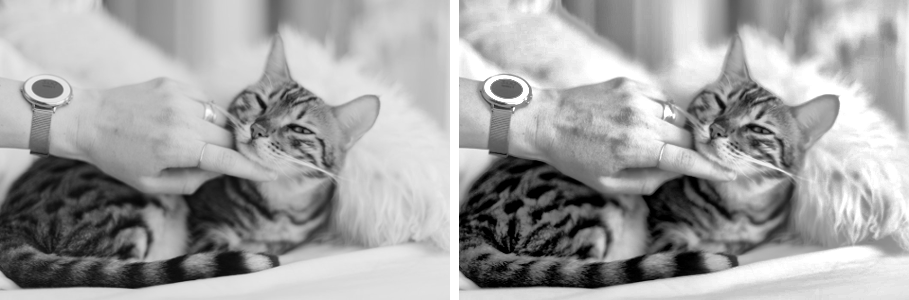
\includegraphics[width=0.95\textwidth]{img/cat.png}
  \caption{Left: input image. Right: sharpened image.}
\end{figure}

The cat's fur on the left-hand side, the person's hand and the cushion on the right-hand side appear to be more detailed.
We observe that the already sharp part of the image on the cat's head stays nice.
We obtained this filter by defining \(f(\Lapl) = -3\Lapl\) in the output image \(z = (I - f(\Lapl))y\).

This corresponds to the adaptive sharpening operator defined in \cite{siam_slides_2016} as \((I + \beta \Lapl)\) with \(\beta > 0\).
This approach remains a simple application of a scalar and doesn't require any eigenvalue computation.
A more complete approach is called multiscale decomposition \cite{talebi_nonlocal_2014} and consists of applying a polynomial function to the Laplacian \(\Lapl\).
We apply different coefficients to different eigenvalues of \(\Lapl\) because each eigenpair captures different features of the image.


\paragraph{Performances and discussions}
We run the algorithm 5 times for each number of processors on the image shown above, up to 192 processors, and average the runs.
Below the total runtime for each number of processors:
\begin{figure}[H]
  \centering
  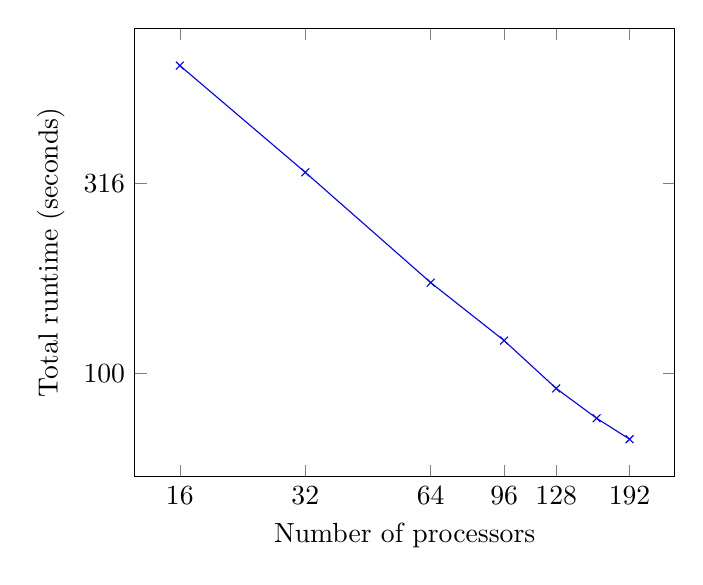
\begin{tikzpicture}
 \begin{axis}[
  xlabel=Number of processors,
  xtick={16, 32, 64, 96, 128, 192},
  xmode=log,
  ymode=log,
  log ticks with fixed point,
  ylabel=Total runtime (seconds)]
   \addplot[color=blue, mark=x] coordinates {
    %(1, )
    %(2, )
    %(4, )
    %(8, )
    (16, 646.344379)
    (32, 338.1412974)
    (64, 173.1325498)
    (96, 121.8080638)
    (128, 91.1042946)
    (160, 76.0524958)
    (192, 66.9623342)
   };
 \end{axis}
\end{tikzpicture}

  \caption{Total runtime of the algorithm with entire matrix computation (log scale).}
\end{figure}

We observe that the runtime decreases significantly with respect to the number of processors.
We can also see that, by doubling the number of processors, we nearly accelerate the runtime by a factor 2.
It is an excellent result since we achieve strong scalability for the entire matrix computation case.
However, some overhead will always be present and the matrix-vector operations necessarily require communication, limiting scalability.
To observe if some parts scale better than others, we compare the proportion of each part:
\begin{figure}[H]
  \centering
  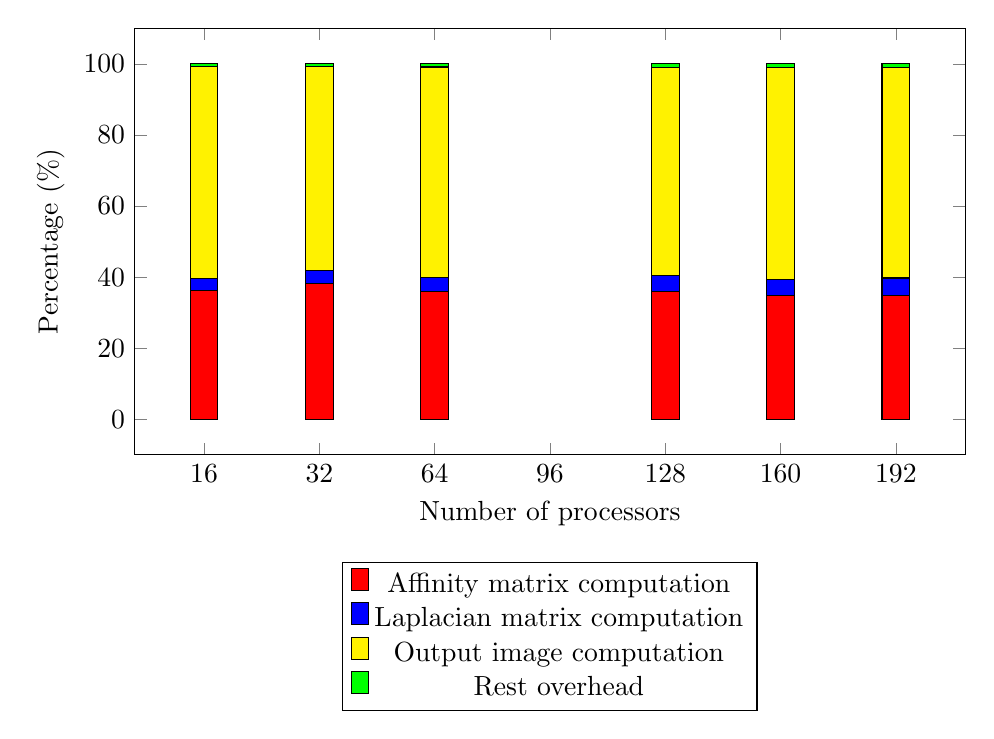
\begin{tikzpicture}
 \begin{axis}[
  ybar stacked,
  height=7cm,
  width=\textwidth,
  xlabel=Number of processors,
  symbolic x coords={
      16, 32, 64, 96, 128, 160, 192
  },
  xtick=data,
  legend style={
   at={(0.5, -0.25)},
   anchor=north
  },
  ylabel={Percentage (\%)}]
  \addplot[ybar, fill=red] plot coordinates {
   (16, 36.11)
   (32, 38.28)
   (64, 36.03)
   (96, 0)
   (128, 36.04)
   (160, 34.73)
   (192, 34.76)};
  \addplot[ybar, fill=blue] plot coordinates {
   (16, 3.62)
   (32, 3.59)
   (64, 3.90)
   (96, 0)
   (128, 4.49)
   (160, 4.71)
   (192, 5)};
  \addplot[ybar, fill=yellow] plot coordinates {
   (16, 59.49)
   (32, 57.32)
   (64, 59.18)
   (96, 0)
   (128, 58.47)
   (160, 59.57)
   (192, 59.21)};
  \addplot[ybar, fill=green] plot coordinates {
   (16, 0.78)
   (32, 0.81)
   (64, 0.89)
   (96, 0)
   (128, 1)
   (160, 1)
   (192, 1.03)};
  \legend{
   Affinity matrix computation,
   Laplacian matrix computation,
   Output image computation,
   Rest overhead}
 \end{axis}
\end{tikzpicture}

  \caption{Proportion of each step in the total execution of the algorithm with entire matrix computation.}
\end{figure}

We see that the proportion of each part remains the same over the increase of processors, meaning that the three main parts scale equivalently.
However, when allocating an excessive amount of processors to this task compared to the input size, we may observe an increase of the runtime because we spend most time on communication overhead.

Overall, computing the entire matrices scales well because we only have matrix-matrix and matrix-vector products.
With an appropriate cluster, those scale nicely.
We now consider larger inputs, which require approximation and introduces linear algebra components which might slow down the algorithm.


\subsection{Approximation computation}

\paragraph{Eigenvalues}
It should be kept in mind that the end of the algorithm, using matrix approximation to compute the filtered image, is not implemented.
Nonetheless, we will present some interesting results about the computation of the eigenvalues of the graph Laplacian operator.
We consider a picture with 402 318 pixels and we sample 1\% of them, which corresponds approximately to 4000 sample pixels.
Additionally to varying the number of processors, we also vary the number of computed eigenvalues from 50 up to 500.
Here are the first 500 eigenvalues of the Laplacian submatrix:

\begin{figure}[H]
  \centering
  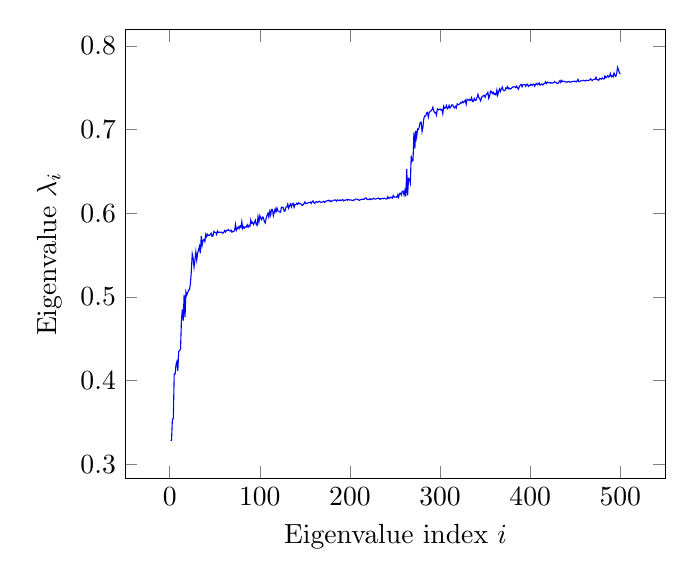
\begin{tikzpicture}
 \begin{axis}[
  xlabel=Eigenvalue index \(i\),
  ylabel=Eigenvalue \(\lambda_i\)]
  \addplot[color=blue] coordinates {
   (1, 0.328403)
   (2, 0.328993)
   (3, 0.354142)
   (4, 0.354558)
   (5, 0.407947)
   (6, 0.407922)
   (7, 0.419087)
   (8, 0.422894)
   (9, 0.411912)
   (10, 0.434953)
   (11, 0.436195)
   (12, 0.437591)
   (13, 0.471408)
   (14, 0.485145)
   (15, 0.471876)
   (16, 0.50277)
   (17, 0.47612)
   (18, 0.506129)
   (19, 0.50255)
   (20, 0.505246)
   (21, 0.508385)
   (22, 0.508875)
   (23, 0.516208)
   (24, 0.530951)
   (25, 0.551366)
   (26, 0.546031)
   (27, 0.535797)
   (28, 0.54417)
   (29, 0.553869)
   (30, 0.544179)
   (31, 0.552599)
   (32, 0.556183)
   (33, 0.560408)
   (34, 0.552089)
   (35, 0.57255)
   (36, 0.561992)
   (37, 0.567683)
   (38, 0.568707)
   (39, 0.566264)
   (40, 0.575036)
   (41, 0.572075)
   (42, 0.574888)
   (43, 0.573638)
   (44, 0.573606)
   (45, 0.574707)
   (46, 0.576157)
   (47, 0.572465)
   (48, 0.572887)
   (49, 0.578266)
   (50, 0.577289)
   (51, 0.577101)
   (52, 0.574753)
   (53, 0.578846)
   (54, 0.577053)
   (55, 0.577171)
   (56, 0.577384)
   (57, 0.577616)
   (58, 0.577029)
   (59, 0.576138)
   (60, 0.577424)
   (61, 0.579389)
   (62, 0.577662)
   (63, 0.579514)
   (64, 0.579413)
   (65, 0.580647)
   (66, 0.579368)
   (67, 0.578908)
   (68, 0.579853)
   (69, 0.577481)
   (70, 0.57841)
   (71, 0.57815)
   (72, 0.579599)
   (73, 0.586778)
   (74, 0.579563)
   (75, 0.581868)
   (76, 0.583686)
   (77, 0.581725)
   (78, 0.584791)
   (79, 0.58317)
   (80, 0.590067)
   (81, 0.58162)
   (82, 0.58403)
   (83, 0.582365)
   (84, 0.583794)
   (85, 0.58359)
   (86, 0.586169)
   (87, 0.583282)
   (88, 0.585467)
   (89, 0.584366)
   (90, 0.592158)
   (91, 0.587962)
   (92, 0.589138)
   (93, 0.586626)
   (94, 0.589144)
   (95, 0.591788)
   (96, 0.586469)
   (97, 0.585384)
   (98, 0.595982)
   (99, 0.589712)
   (100, 0.597098)
   (101, 0.593938)
   (102, 0.59224)
   (103, 0.595483)
   (104, 0.594726)
   (105, 0.59026)
   (106, 0.588475)
   (107, 0.593881)
   (108, 0.597248)
   (109, 0.600065)
   (110, 0.595491)
   (111, 0.60219)
   (112, 0.597753)
   (113, 0.604718)
   (114, 0.604648)
   (115, 0.597022)
   (116, 0.601191)
   (117, 0.605243)
   (118, 0.601688)
   (119, 0.606338)
   (120, 0.602887)
   (121, 0.602497)
   (122, 0.601607)
   (123, 0.601351)
   (124, 0.60732)
   (125, 0.606745)
   (126, 0.606653)
   (127, 0.602445)
   (128, 0.602744)
   (129, 0.607308)
   (130, 0.607352)
   (131, 0.610958)
   (132, 0.606089)
   (133, 0.609026)
   (134, 0.611262)
   (135, 0.607655)
   (136, 0.611064)
   (137, 0.611929)
   (138, 0.607066)
   (139, 0.610522)
   (140, 0.610409)
   (141, 0.611942)
   (142, 0.610808)
   (143, 0.612479)
   (144, 0.611327)
   (145, 0.611731)
   (146, 0.610665)
   (147, 0.609294)
   (148, 0.609987)
   (149, 0.611622)
   (150, 0.613529)
   (151, 0.611501)
   (152, 0.611571)
   (153, 0.612294)
   (154, 0.612613)
   (155, 0.612933)
   (156, 0.613407)
   (157, 0.611578)
   (158, 0.613732)
   (159, 0.614805)
   (160, 0.612629)
   (161, 0.61192)
   (162, 0.61353)
   (163, 0.613907)
   (164, 0.613104)
   (165, 0.613565)
   (166, 0.614426)
   (167, 0.613664)
   (168, 0.613054)
   (169, 0.613152)
   (170, 0.613743)
   (171, 0.614392)
   (172, 0.613066)
   (173, 0.614177)
   (174, 0.614879)
   (175, 0.614939)
   (176, 0.61559)
   (177, 0.614663)
   (178, 0.615456)
   (179, 0.613848)
   (180, 0.614737)
   (181, 0.614914)
   (182, 0.615532)
   (183, 0.616009)
   (184, 0.615817)
   (185, 0.614419)
   (186, 0.615941)
   (187, 0.615559)
   (188, 0.615346)
   (189, 0.61598)
   (190, 0.615062)
   (191, 0.615785)
   (192, 0.616532)
   (193, 0.614875)
   (194, 0.615483)
   (195, 0.615767)
   (196, 0.61628)
   (197, 0.615569)
   (198, 0.616636)
   (199, 0.616125)
   (200, 0.615727)
   (201, 0.616041)
   (202, 0.615556)
   (203, 0.615182)
   (204, 0.615932)
   (205, 0.615761)
   (206, 0.616798)
   (207, 0.616999)
   (208, 0.616871)
   (209, 0.616434)
   (210, 0.615357)
   (211, 0.61592)
   (212, 0.616345)
   (213, 0.616586)
   (214, 0.616894)
   (215, 0.616613)
   (216, 0.616905)
   (217, 0.618205)
   (218, 0.618257)
   (219, 0.616599)
   (220, 0.616334)
   (221, 0.616325)
   (222, 0.617383)
   (223, 0.616319)
   (224, 0.617059)
   (225, 0.617017)
   (226, 0.617999)
   (227, 0.617267)
   (228, 0.616927)
   (229, 0.617276)
   (230, 0.617597)
   (231, 0.617804)
   (232, 0.618269)
   (233, 0.616643)
   (234, 0.617436)
   (235, 0.617211)
   (236, 0.617794)
   (237, 0.617264)
   (238, 0.618154)
   (239, 0.617462)
   (240, 0.617177)
   (241, 0.617079)
   (242, 0.619852)
   (243, 0.617906)
   (244, 0.618103)
   (245, 0.619186)
   (246, 0.619102)
   (247, 0.61813)
   (248, 0.621239)
   (249, 0.619201)
   (250, 0.619493)
   (251, 0.619594)
   (252, 0.61895)
   (253, 0.621864)
   (254, 0.619021)
   (255, 0.623788)
   (256, 0.623924)
   (257, 0.621764)
   (258, 0.626421)
   (259, 0.626401)
   (260, 0.621975)
   (261, 0.627299)
   (262, 0.620112)
   (263, 0.652731)
   (264, 0.621314)
   (265, 0.641508)
   (266, 0.640666)
   (267, 0.636291)
   (268, 0.66886)
   (269, 0.662238)
   (270, 0.663165)
   (271, 0.696515)
   (272, 0.677108)
   (273, 0.69828)
   (274, 0.690668)
   (275, 0.700609)
   (276, 0.700017)
   (277, 0.703813)
   (278, 0.708642)
   (279, 0.70895)
   (280, 0.697594)
   (281, 0.702937)
   (282, 0.713406)
   (283, 0.716234)
   (284, 0.716115)
   (285, 0.7198)
   (286, 0.720496)
   (287, 0.714957)
   (288, 0.720204)
   (289, 0.721803)
   (290, 0.722229)
   (291, 0.723694)
   (292, 0.72654)
   (293, 0.722341)
   (294, 0.720151)
   (295, 0.720461)
   (296, 0.71714)
   (297, 0.724678)
   (298, 0.723453)
   (299, 0.723952)
   (300, 0.724578)
   (301, 0.723302)
   (302, 0.724001)
   (303, 0.718818)
   (304, 0.727797)
   (305, 0.725351)
   (306, 0.725868)
   (307, 0.72881)
   (308, 0.7249)
   (309, 0.725978)
   (310, 0.728913)
   (311, 0.725651)
   (312, 0.726962)
   (313, 0.729484)
   (314, 0.729512)
   (315, 0.7271)
   (316, 0.725885)
   (317, 0.727652)
   (318, 0.725808)
   (319, 0.730581)
   (320, 0.729557)
   (321, 0.73004)
   (322, 0.730756)
   (323, 0.732401)
   (324, 0.731684)
   (325, 0.733546)
   (326, 0.73228)
   (327, 0.73343)
   (328, 0.735144)
   (329, 0.730156)
   (330, 0.736182)
   (331, 0.735642)
   (332, 0.734628)
   (333, 0.736054)
   (334, 0.734991)
   (335, 0.73812)
   (336, 0.733373)
   (337, 0.733805)
   (338, 0.737036)
   (339, 0.734852)
   (340, 0.735032)
   (341, 0.738114)
   (342, 0.742074)
   (343, 0.738399)
   (344, 0.736564)
   (345, 0.734353)
   (346, 0.738659)
   (347, 0.739091)
   (348, 0.740611)
   (349, 0.740995)
   (350, 0.738616)
   (351, 0.741615)
   (352, 0.742678)
   (353, 0.744339)
   (354, 0.737261)
   (355, 0.739999)
   (356, 0.745976)
   (357, 0.74539)
   (358, 0.743067)
   (359, 0.74462)
   (360, 0.741842)
   (361, 0.742852)
   (362, 0.741281)
   (363, 0.747162)
   (364, 0.741006)
   (365, 0.74558)
   (366, 0.748506)
   (367, 0.745377)
   (368, 0.748645)
   (369, 0.75072)
   (370, 0.747139)
   (371, 0.746351)
   (372, 0.746547)
   (373, 0.749818)
   (374, 0.748981)
   (375, 0.75129)
   (376, 0.748655)
   (377, 0.749352)
   (378, 0.748317)
   (379, 0.749113)
   (380, 0.750187)
   (381, 0.751118)
   (382, 0.750899)
   (383, 0.75122)
   (384, 0.750024)
   (385, 0.751781)
   (386, 0.749717)
   (387, 0.748168)
   (388, 0.751288)
   (389, 0.7532)
   (390, 0.753793)
   (391, 0.750979)
   (392, 0.753583)
   (393, 0.753691)
   (394, 0.75375)
   (395, 0.751578)
   (396, 0.753477)
   (397, 0.754161)
   (398, 0.751536)
   (399, 0.752857)
   (400, 0.752527)
   (401, 0.754162)
   (402, 0.7529)
   (403, 0.753956)
   (404, 0.754121)
   (405, 0.751759)
   (406, 0.754159)
   (407, 0.755096)
   (408, 0.753618)
   (409, 0.754439)
   (410, 0.755523)
   (411, 0.753051)
   (412, 0.753854)
   (413, 0.754381)
   (414, 0.753288)
   (415, 0.75462)
   (416, 0.754951)
   (417, 0.756929)
   (418, 0.754855)
   (419, 0.756627)
   (420, 0.756008)
   (421, 0.755664)
   (422, 0.756235)
   (423, 0.755252)
   (424, 0.755887)
   (425, 0.755456)
   (426, 0.756151)
   (427, 0.757361)
   (428, 0.756083)
   (429, 0.755992)
   (430, 0.755037)
   (431, 0.755263)
   (432, 0.756811)
   (433, 0.758444)
   (434, 0.756257)
   (435, 0.758722)
   (436, 0.757174)
   (437, 0.757314)
   (438, 0.757707)
   (439, 0.756797)
   (440, 0.756883)
   (441, 0.756531)
   (442, 0.757291)
   (443, 0.757449)
   (444, 0.756491)
   (445, 0.756641)
   (446, 0.757202)
   (447, 0.757592)
   (448, 0.757287)
   (449, 0.757687)
   (450, 0.757621)
   (451, 0.756988)
   (452, 0.757984)
   (453, 0.759911)
   (454, 0.757089)
   (455, 0.757452)
   (456, 0.758165)
   (457, 0.758075)
   (458, 0.75864)
   (459, 0.758848)
   (460, 0.758345)
   (461, 0.757997)
   (462, 0.758895)
   (463, 0.758766)
   (464, 0.758405)
   (465, 0.758796)
   (466, 0.759189)
   (467, 0.760668)
   (468, 0.759334)
   (469, 0.758513)
   (470, 0.759774)
   (471, 0.759898)
   (472, 0.759872)
   (473, 0.762496)
   (474, 0.759706)
   (475, 0.759454)
   (476, 0.758765)
   (477, 0.76111)
   (478, 0.760817)
   (479, 0.760114)
   (480, 0.761605)
   (481, 0.760502)
   (482, 0.760392)
   (483, 0.764116)
   (484, 0.761848)
   (485, 0.762582)
   (486, 0.764355)
   (487, 0.762644)
   (488, 0.763692)
   (489, 0.766856)
   (490, 0.763033)
   (491, 0.764073)
   (492, 0.762971)
   (493, 0.76745)
   (494, 0.764525)
   (495, 0.763494)
   (496, 0.767313)
   (497, 0.774561)
   (498, 0.771342)
   (499, 0.768007)
   (500, 0.766166)
  };
 \end{axis}
\end{tikzpicture}

  \caption{First 500 eigenvalues \(\lambda_i\) of the Laplacian submatrix.}
  \label{fig:500_eigenvalues}
\end{figure}

To compute the eigenvalues in figure \ref{fig:500_eigenvalues}, we used the inverse subspace iteration \cite{el_khoury_acceleration_2014}.
We now look at the algorithm runtime performances.


\paragraph{Performances}
As a reminder, we used GMRES to solve the linear systems with RAS preconditioning and using GMRES on the subdomains.
We sample 1\% of the pixels of an image with \(4 \cdot 10^5\) pixels using spatially uniform sampling.
The performances of the inverse subspace iteration for 50 and 500 eigenvalues:

\begin{figure}[H]
 \centering
 \begin{tikzpicture}
 \begin{groupplot}[
  group style={
   group size=2 by 1,
   xlabels at=edge bottom,
   ylabels at=edge left,
   horizontal sep=1.5cm,
   },
  height=6cm,
  width=0.5\textwidth,
  xlabel=Number of processors,
  xtick={2, 4, 8, 16, 32, 64, 128},
  xmode=log,
  ymode=log,
  log ticks with fixed point,
  ylabel=Runtime (seconds)
  ]
  \nextgroupplot[title={50 eigenvalues.}]
   \addplot[color=blue, mark=x] coordinates {
    (2, 772.1529408)
    (4, 381.4875584)
    (8, 196.6197338)
    (16, 104.6891928)
    (32, 59.8903464)
    (64, 35.9956886)
    (96, 29.214667)
    (128, 25.4793632)
    (160, 24.0418716)
    (192, 23.1824056)
   };

  \nextgroupplot[title={500 eigenvalues.}]
   \addplot[color=blue, mark=x] coordinates {
    (2, 7149.885403)
    (4, 5149.912356)
    (8, 4373.481026)
    (16, 3903.60577)
    (32, 3803.859549)
    (64, 3712.591258)
    (96, 3824.621957)
    (128, 3939.533307)
    (160, 3986.572888)
    (192, 4383.063958)
   };
 \end{groupplot}
\end{tikzpicture}

 \caption{Runtime of the inverse subspace iteration part of the algorithm (log scale).}
 \label{fig:inv_it_runtime}
\end{figure}

When increasing a low number of processors, we see an improvement of the performances in both cases of figure \ref{fig:inv_it_runtime}.
But the runtime stagnates slowly for 50 eigenvalues and quickly for 500 eigenvalues.
We even observe a raise of the runtime for 500 eigenvalues.
The algorithm reaches its parallelisation limit and the communication overhead takes over.
For 500 eigenvalues, the runtime for 2 processors is over 7000 seconds, and the fastest runtime is reached for 64 processors and is of 3700 seconds.

We know that the inverse iteration part of the algorithm is not scaling correctly compared to the other parts.
For any amount of computed eigenvalues, when we increase the number of processes, the proportion of time spent computing the eigenvalues increases.
For 500 eigenvalues and 128 processors, we spend more than 99\% of the time computing the eigenvalues.
This confirms that the algorithm does not quite scale yet.

We look at the internal steps of the inverse power method to see where lies the problem.
The algorithm consists of iteratively solving \(m\) linear systems, orthonormalising the vectors and computing the residual norm.
Here is the proportion of each step of the inverse subspace interation for the computation of 50 and 500 eigenvalues:

\begin{figure}[H]
 \centering
 \begin{tikzpicture}
 \begin{groupplot}[
  group style={
   group size=2 by 1,
   xlabels at=edge bottom,
   ylabels at=edge left,
   },
  ybar stacked,
  ymin=0,
  ymax=100,
  height=7cm,
  width=0.5\textwidth,
  xlabel=Number of processors,
  ylabel={Percentage (\%)},
  symbolic x coords={2, 4, 8, 16, 32, 64, 96, 128, 160, 192},
  legend style={
   at={(0, -0.25)},
   anchor=north}
  ]
  \nextgroupplot[title={50 eigenvalues.}]
  \addplot[ybar, fill=blue] plot coordinates {
   (2, 8.14)
   (4, 6.16)
   (8, 5.98)
   (16, 9.09)
   (32, 13.50)
   (64, 18.56)
   (96, 22.42)
   (128, 25.35)
   (160, 27.53)
   (192, 29.06)};
  \addplot[ybar, fill=red] plot coordinates {
   (2, 0.46)
   (4, 0.96)
   (8, 2.01)
   (16, 3.90)
   (32, 7.31)
   (64, 13.29)
   (96, 17.61)
   (128, 20.94)
   (160, 23.90)
   (192, 26.27)};
  \addplot[ybar, fill=yellow] plot coordinates {
   (2, 85.67)
   (4, 86.96)
   (8, 86.16)
   (16, 81.40)
   (32, 73.91)
   (64, 63.23)
   (96, 55.21)
   (128, 49.07)
   (160, 43.95)
   (192, 40.00)};
  \addplot[ybar, fill=green] plot coordinates {
   (2, 5.74)
   (4, 5.92)
   (8, 5.84)
   (16, 5.61)
   (32, 5.28)
   (64, 4.91)
   (96, 4.76)
   (128, 4.64)
   (160, 4.62)
   (192, 4.68)};

  \nextgroupplot[title={500 eigenvalues.}]
  \addplot[ybar, fill=blue] plot coordinates {
   (2, 23.76)
   (4, 15.29)
   (8, 11.43)
   (16, 12.30)
   (32, 11.68)
   (64, 9.84)
   (96, 9.47)
   (128, 9.75)
   (160, 9.57)
   (192, 9.39)};
  \addplot[ybar, fill=red] plot coordinates {
   (2, 46.02)
   (4, 63.07)
   (8, 75.14)
   (16, 79.65)
   (32, 83.37)
   (64, 86.81)
   (96, 87.72)
   (128, 87.77)
   (160, 88.07)
   (192, 88.50)};
  \addplot[ybar, fill=yellow] plot coordinates {
   (2, 28.78)
   (4, 20.15)
   (8, 11.97)
   (16, 6.60)
   (32, 3.49)
   (64, 1.84)
   (96, 1.29)
   (128, 0.98)
   (160, 0.80)
   (192, 0.64)};
  \addplot[ybar, fill=green] plot coordinates {
   (2, 1.44)
   (4, 1.48)
   (8, 1.46)
   (16, 1.46)
   (32, 1.46)
   (64, 1.51)
   (96, 1.53)
   (128, 1.50)
   (160, 1.56)
   (192, 1.47)};
  \legend{
   Solving the system of linear equations,
   Gram-Schmidt orthogonalisation,
   Residual norm computation,
   Rest overhead}
 \end{groupplot}
\end{tikzpicture}

 \caption{Proportion of each step in the inverse subspace iteration.}
 \label{fig:inv_it_proportion}
\end{figure}

We observe from figure \ref{fig:inv_it_proportion} that the Gram-Schmidt orthogonalisation is the limiting factor and is the most time-consuming step of the inverse iteration as the number of processors grows.
It is a well-known problem that the simple Gram-Schmidt process is actually difficult to parallelise efficiently.
Small optimisations for a parallel Gram-Schmidt orthogonalisation exist \cite{katagiri_parallel_gram_schmidt_2003} but they do not properly solve the problem.
This issue will be difficult to overcome completely.


\paragraph{Skipping some orthogonalisations}
Fundamentally, the orthogonalisation is used to stabilise the algorithm.
To accelerate our algorithm further, we try to orthogonalise the vectors \(X_k\) every other iteration instead of every iteration.
We present below the resulting performances:

\begin{figure}[H]
  \centering
  \begin{tikzpicture}
 \begin{groupplot}[
  group style={
   group size=2 by 1,
   xlabels at=edge bottom,
   ylabels at=edge left,
   horizontal sep=1.5cm,
   },
  height=6cm,
  width=0.5\textwidth,
  xlabel=Number of processors,
  xtick={2, 4, 8, 16, 32, 64, 128},
  xmode=log,
  ymode=log,
  log ticks with fixed point,
  ylabel=Runtime (seconds)
  ]
  \nextgroupplot[title={50 eigenvalues.}]
   \addplot[color=blue, mark=x] coordinates {
    (2, 819.1718588)
    (4, 404.5779052)
    (8, 207.887785)
    (16, 109.2656354)
    (32, 61.5224218)
    (64, 35.5858806)
    (96, 28.0760846)
    (128, 24.3417164)
    (160, 22.365463)
    (192, 21.1874868)
   };

  \nextgroupplot[title={500 eigenvalues.}]
   \addplot[color=blue, mark=x] coordinates {
    (2, 5613.950337)
    (4, 3614.57139)
    (8, 2804.417351)
    (16, 2346.925115)
    (32, 2223.999989)
    (64, 2104.544023)
    (96, 2148.624336)
    (128, 2264.674778)
    (160, 2226.515463)
    (192, 2494.121987)
   };
 \end{groupplot}
\end{tikzpicture}

  \caption{Runtime of the inverse subspace iteration with skipping the Gram-Schmidt procedure every other iteration (log scale).}
\end{figure}

The performances for 50 eigenvalues are similar to the case when we are not skipping the Gram-Schmidt orthogonalisation every other iteration.
We saw that only a small proportion of time is spent doing the orthogonalisation in this case, so the impact is not significant.

However, for computing 500 eigenvalues, the runtime with skipping the orthogonalisation every other iteration is much lower.
Most time is spent doing the Gram-Schmidt process, so the execution is considerably sped up.
For 2 processors, the runtime is around 5600 seconds and the fastest runtime is 2100 seconds for 64 processors.
Even if the algorithm requires a few more outer iterations to converge, we nearly observe a factor 2 speed up with respect to the algorithm without skipping the Gram-Schmidt procedure.
The communication overhead of the method remains a problem when the number of processors is large.

When skipping the Gram-Schmidt more often than every other iteration, we might see further improvements.
Below the runtime for 2 and 64 processors of the inverse subspace algorithm depending on the frequency of orthogonalisation:

\begin{figure}[H]
  \centering
  \begin{tikzpicture}
 \begin{groupplot}[
  group style={
   group size=2 by 1,
   xlabels at=edge bottom,
   ylabels at=edge left,
   horizontal sep=2.2cm,
   },
  height=6cm,
  width=0.5\textwidth,
  xlabel={Orthogonalisation every \(x\) iterations},
  xtick={1, 2, 3, 4, 5},
  %xmode=log,
  %ymode=log,
  %log ticks with fixed point,
  ylabel=Runtime (seconds),
  legend style={
   at={(1, -0.3)},
   anchor=north
  },
  ]
  \nextgroupplot[title={2 processors, 500 eigenvalues.}]
   \addplot[color=blue, mark=x] coordinates {
    (1, 7149.885403)
    (2, 5613.950337)
    (3, 0)
    (4, 0)
    (5, 0)
   };
   \addlegendentry{Runtime}
   \addplot[color=black, domain=1:5, dashed] expression {
    7149.885403/x};
   \addlegendentry{Linear speedup}

  \nextgroupplot[title={64 processors, 500 eigenvalues.}]
   \addplot[color=blue, mark=x] coordinates {
    (1, 3712.591258)
    (2, 2104.544023)
    (3, 0)
    (4, 0)
    (5, 0)
   };
   \addplot[color=black, domain=1:5, dashed] expression {
    3712.591258/x};
 \end{groupplot}
\end{tikzpicture}


  \caption{Runtime of the inverse subspace iteration depending on the amount of Gram-Schmidt procedures.}
\end{figure}

For 2 processors, we see that the speedup stagnates quickly when skipping the Gram-Schmidt orthogonalisation more and more often.
Indeed, the orthogonalisation represents a decent proportion of the execution time for 2 processors whereas it represents over 85\% for 64 processors.
Therefore we observe a speedup of the inverse subspace iteration that is nearly linear for 64 processors.
The number of outer iterations between not skipping the Gram-Schmidt algorithm and applying it every 5 iterations only varies from 38 to 40 which explains the resulting runtime.


\paragraph{SLEPc comparison}
We compare the performances of our algorithm with the parallel eigenvalue problem solver SLEPc.
We compute the same amount of eigenvalues with the same number of processors using the provided Krylov-Schur algorithm \cite{stewart_krylovschur_2002}.
The performances of SLEPc in comparison of our method:

\begin{figure}[H]
  \centering
  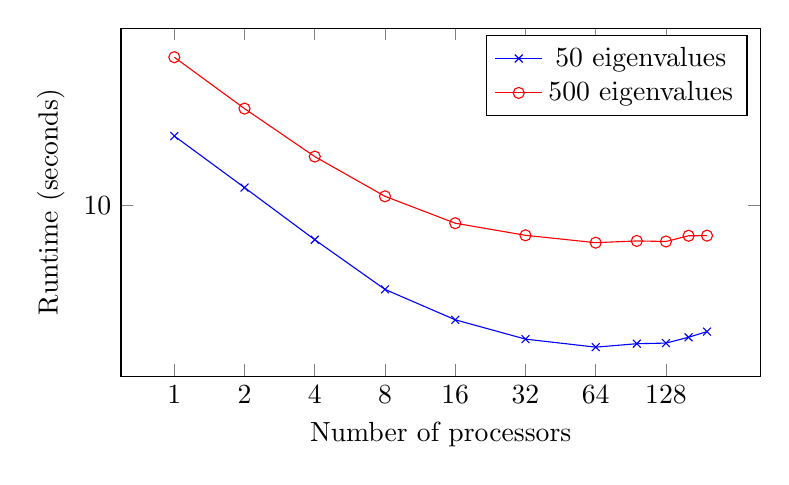
\begin{tikzpicture}
 \begin{axis}[
  height=6cm,
  width=0.8\textwidth,
  xlabel=Number of processors,
  xtick={1, 2, 4, 8, 16, 32, 64, 128},
  xmode=log,
  ymode=log,
  log ticks with fixed point,
  ylabel=Runtime (seconds)]
   \addplot[color=blue, mark=x] coordinates {
    (1, 22.2659924)
    (2, 12.2595888)
    (4, 6.7051142)
    (8, 3.7737956)
    (16, 2.6544356)
    (32, 2.1228378)
    (64, 1.9344542)
    (96, 2.0126992)
    (128, 2.027464)
    (160, 2.1684376)
    (192, 2.3157606)
   };
   \addlegendentry{50 eigenvalues}
   \addplot[color=red, mark=o] coordinates {
    (1, 55.4115932)
    (2, 30.5698838)
    (4, 17.5465694)
    (8, 11.081354)
    (16, 8.1181468)
    (32, 7.0558288)
    (64, 6.4795788)
    (96, 6.6119022)
    (128, 6.5703108)
    (160, 7.0204188)
    (192, 7.0297304)
   };
   \addlegendentry{500 eigenvalues}
 \end{axis}
\end{tikzpicture}

  \caption{Runtime of the Krylov-Schur algorithm in SLEPc (log scale).}
\end{figure}

First of all, it is notable that both execution times for 50 and 500 eigenvalues are close to each other.
This comes from the way the internal Krylov-Schur algorithm functions.
%It has to compute multiple eigenpairs and then discard the unwanted ones, meaning that the method can have the same performances for different amounts of requested eigenvalues.

The algorithm, on this test case, is faster than our implementation.
However, both approaches tend to have a light increase in the runtime after reaching a certain number of processors.


\paragraph{Linear solver performances}
\paragraph{}
We want to explore the behavior of the used linear solver using domain decomposition methods for our inverse iteration algorithm.
We reming that we used GMRES and domain decomposition method RAS with 2 domains per process for the previous examples.
We compare the runtimes of solving 50 linear systems with different number of processors, for different solvers with and without preconditioner:

\begin{figure}[H]
 \centering
 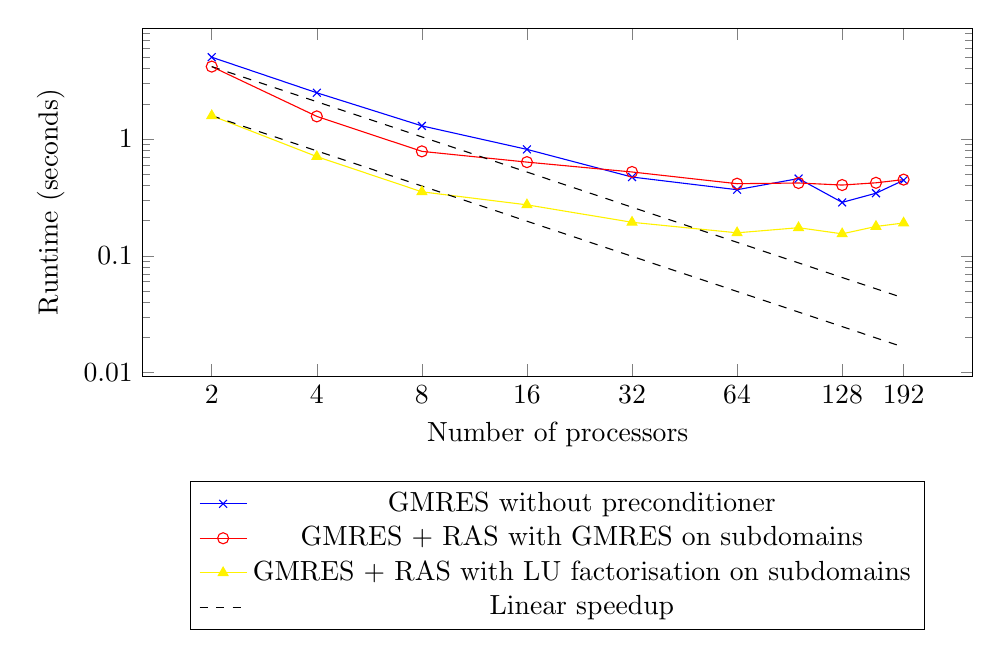
\begin{tikzpicture}
 \begin{axis}[
  height=6cm,
  width=\textwidth,
  xlabel=Number of processors,
  xtick={2, 4, 8, 16, 32, 64, 128, 192},
  xmode=log,
  ymode=log,
  log ticks with fixed point,
  ylabel=Runtime (seconds),
  legend style={
   at={(0.5, -0.3)},
   anchor=north
  }]
   \addplot[color=blue, mark=x] coordinates {
    (2, 5.019035956)
    (4, 2.489311578)
    (8, 1.295918689)
    (16, 0.8153684889)
    (32, 0.4725504889)
    (64, 0.3680468222)
    (96, 0.4586239333)
    (128, 0.2866520667)
    (160, 0.3435106444)
    (192, 0.4434605778)
   };
   \addlegendentry{GMRES without preconditioner}
   \addplot[color=red, mark=o] coordinates {
    (2, 4.171304311)
    (4, 1.562855289)
    (8, 0.78404696)
    (16, 0.6342229867)
    (32, 0.5220878222)
    (64, 0.4143123111)
    (96, 0.4201508889)
    (128, 0.4034540222)
    (160, 0.4217084444)
    (192, 0.4490838667)
   };
   \addlegendentry{GMRES + RAS with GMRES on subdomains}
   \addplot[color=yellow, mark=triangle*] coordinates {
    (2, 1.583247378)
    (4, 0.7071820222)
    (8, 0.3530209556)
    (16, 0.2730702667)
    (32, 0.193635)
    (64, 0.1572552667)
    (96, 0.1740185111)
    (128, 0.1541527111)
    (160, 0.1782941778)
    (192, 0.1908772667)
   };
   \addlegendentry{GMRES + RAS with LU factorisation on subdomains}
   \addplot[color=black, domain=2:192, dashed] expression {
    4.171304311*2/x};
   \addlegendentry{Linear speedup}
   \addplot[color=black, domain=2:192, dashed] expression {
    1.583247378*2/x};
 \end{axis}
\end{tikzpicture}

 \caption{Runtime of the linear solver for 50 eigenvalues.}
\end{figure}

Overall, we observe that using a domain decomposition method as preconditioner for our dense systems shows slightly better runtime performances.
Between not using a preconditioner and applying domain decomposition with GMRES on the subdomains, the difference is visible for a small number of processors.
When increasing the number of processors, both tend to have the same performances, so preconditioning takes the same time as solving the system with an ill-conditioned matrix.

Applying the LU factorisation on the subdomains exposes a much better runtime.
Indeed, the input matrix is rather small in our case, and by splitting the problems into subdomains, the matrices are even smaller and suitable for a direct method.

For all methods, the speedup is nearly linear until 8 processors and we see a stagnation of the runtime after.

